\section{总体概述}\label{sec:General_Description}

\subsection{产品背景}

\subsubsection{概述}

随着现代生活方式的转变,宠物已逐渐成为许多家庭的重要成员。根据行业数据,全球宠物市场的规模近年来呈现出快速增长的趋势,特别是在中国,宠物经济正在崛起。越来越多的人选择养宠物,不仅为了陪伴,还为了精神上的寄托与互动体验。人们对宠物健康、护理、训练、娱乐等各方面的关注度持续上升,这催生了对优质宠物服务平台的强烈需求。

此外,数字化和智能化技术的发展为宠物行业带来了新的机遇。宠物主人越来越希望通过网站平台,方便地获取宠物相关的信息,并享受便捷的线上服务,如参与宠物社区讨论、获取最新的宠物新闻、发布和浏览宠物领养信息等。

PetJoy 通过提供在线社区、实时新闻更新、宠物领养信息发布,以及基于人工智能的宠物助理服务等,为宠物爱好者打造了一个一站式的数字化平台。

\subsubsection{产品核心功能}
\begin{itemize}
\item \textbf{用户和通知}:用户和通知模块负责维护用户的基本信息和用户间的互动,同时也管理着系统对用户的各类通知。该模块通过一系列的表单和功能设计,确保用户信息的安全存储、隐私设置的灵活性以及用户间高效便捷的沟通。用户可以设置自己的个人信息,包括但不限于头像、昵称、性别、生日等,以及隐私控制选项,如公开或隐藏特定信息。此外,通知系统能够显示用户收到的各类互动消息,帮助用户及时了解他人与自己的互动情况。
 \item \textbf{宠物社区}:用户可以在社区中分享宠物的日常生活,发布宠物照片等,参与宠物相关的讨论和话题,建立起与其他宠物爱好者的联系和互动。社区通过帖子表记录用户发布的帖子及互动数据,如点赞、评论和收藏等,衡量内容受欢迎程度,提高用户满意度。帖子分类确保内容的有效管理和组织,便于用户发现感兴趣的话题。评论功能支持用户间的互动交流,增强了讨论的深度和广度。收藏功能让用户保存喜欢的内容,便于日后查看,并为平台提供宝贵的用户兴趣数据。
    \item \textbf{宠物新闻}:平台提供最新的宠物相关新闻和资讯,涵盖宠物健康、宠物护理、宠物训练等各个领域,帮助用户实时掌握宠物行业的动态和趋势。我们通过新闻表和新闻标签表构建了一个内容发布和管理系统。新闻标签帮助用户根据兴趣快速筛选新闻,增强内容的可发现性。新闻表记录新闻详情及用户互动数据,如点赞、点踩、评论等,用户可在新闻评论表中发表看法,增加内容深度和互动性。
    \item \textbf{宠物领养}:它详细记录了每只可供领养宠物的信息,包括名称、年龄、品种、健康状况、位置及领养状态等,通过记录特殊护理需求、饮食习惯等细节,平台提高了宠物的领养率,并确保宠物找到最适合的新家,为有意领养宠物的用户提供一个安全可靠的渠道。用户可以浏览各类可供领养的宠物信息,了解宠物的背景、健康状况等,方便用户做出合适的领养决定。
    \item \textbf{宠物百科}:提供详尽的宠物知识库,涵盖各种宠物的养护知识、品种介绍、常见问题解答等,通过宠物分类表和子类表帮助用户快速找到感兴趣的宠物类型及其具体品种。每个品种介绍包括起源、体型、毛色、寿命、性格和饮食习惯等,帮助用户深入了解不同品种的特征,为选择和护理宠物提供实用参考。直观的图片和文字描述相结合,使用户能全面了解每个品种的特点,进而做出更加符合个人情况的选择。帮助宠物新手和有经验的饲主更好地照顾自己的宠物。
    \item \textbf{宠物AI}:通过调用接口,引入人工智能技术,为用户提供智能化的宠物服务,如宠物的行为解释、健康建议等,提升用户的养宠体验。通过简洁易用的界面,用户可以输入宠物的相关信息或问题,AI助理会基于大数据给出评估和建议。这一功能大大提升了用户的养宠体验,特别是在遇到一般性或常见问题时,AI助理可以快速给予回复,帮助用户更好地照顾他们的宠物。
\end{itemize}

我们的核心工程涵盖了从前端界面的设计到后端系统的架构,确保平台的稳定性、易用性和扩展性。在前端方面,PetJoy 前端应用程序基于 Vue3.js 渐进式框架和 Element Plus 组件库实现,采用响应式设计和流畅的用户交互,确保用户在各种设备上都能获得一致的体验。后端开发则使用 C\# 和 ASP.NET Core 架构,并结合 Entity Framework Core 进行 ROM 访问,构建了一个高效、稳定的系统,支持大规模用户的并发访问,并确保数据的安全和操作的顺畅。在人工智能模块方面,我们通过调用接口,集成了智能助理服务,帮助用户解决与宠物相关的问题。整个项目的工程设计围绕用户体验和技术可扩展性展开,确保平台能够不断适应市场变化和用户需求的升级。

\subsubsection{市场驱动因素}

\paragraph{市场需求}

在当前宠物市场快速发展的背景下,各类需求不断涌现,推动了整个行业的多样化和精细化发展。以下是几大主要的市场需求分析:

\begin{enumerate}
    \item \textbf{宠物市场逐渐扩大,前景广阔}

    近年来,随着人们生活水平的不断提高,宠物市场呈现出快速增长的态势。越来越多的人选择将宠物纳入家庭的一员,与宠物建立深厚的情感纽带。宠物的种类也日趋丰富,从传统的猫、狗,到鸟类、爬行动物等,都受到了人们的喜爱。宠物的消费领域也逐渐扩大,涵盖了食品、玩具、服装、医疗等多个方面,形成了一个庞大的产业链。
    
	\begin{figure}[htbp]
		\centering
		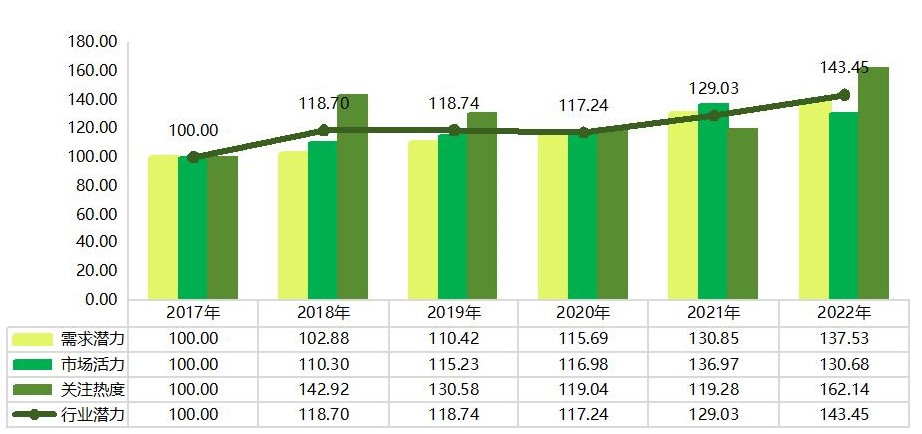
\includegraphics[scale=0.6]{PetDevelopmentReport.jpg}
		\caption{中国宠物行业发展指数报告(2023)}
		\label{PetDevelopmentReport}
	\end{figure}

    \item \textbf{情感共鸣成为养宠人士的重要诉求,宠物“家人化”趋势愈加明显}
    
    在快节奏、高压力的现代生活中,宠物成为了人们寻求情感寄托和陪伴的重要对象。养宠人士与宠物之间建立起了深厚的情感联系,宠物不再仅仅是生活中的一个玩伴,更是成为了家庭成员的一部分。但目前宠物与主人互动方式单一。虽然宠物主人与宠物之间有着深厚的情感联系,但现有的互动方式往往局限于日常陪伴和简单的游戏。缺乏更多元化、更具创意的互动方式,使得宠物主人在忙碌的生活中难以充分表达对宠物的关爱。

	\begin{figure}[htbp]
	\centering
	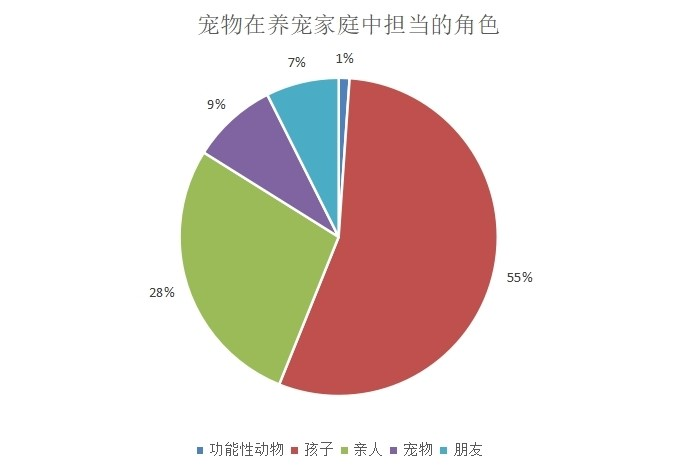
\includegraphics[scale=1]{PetRole.jpg}
	\caption{宠物在养宠家庭中担当的角色(数据来源:MobData研究院)}
	\label{PetRole}
	\end{figure} 
	
    \item \textbf{养宠理念升级,健康养成为趋势}
    
    随着宠物市场的蓬勃发展,养宠理念也在逐渐升级,健康养宠已成为一种新兴趋势。越来越多的宠物主人开始认识到,宠物不仅仅是生活中的陪伴者,更是家庭的一员,需要得到全方位、精细化的照顾。
 
 	\begin{figure}[htbp]
 	\centering
 	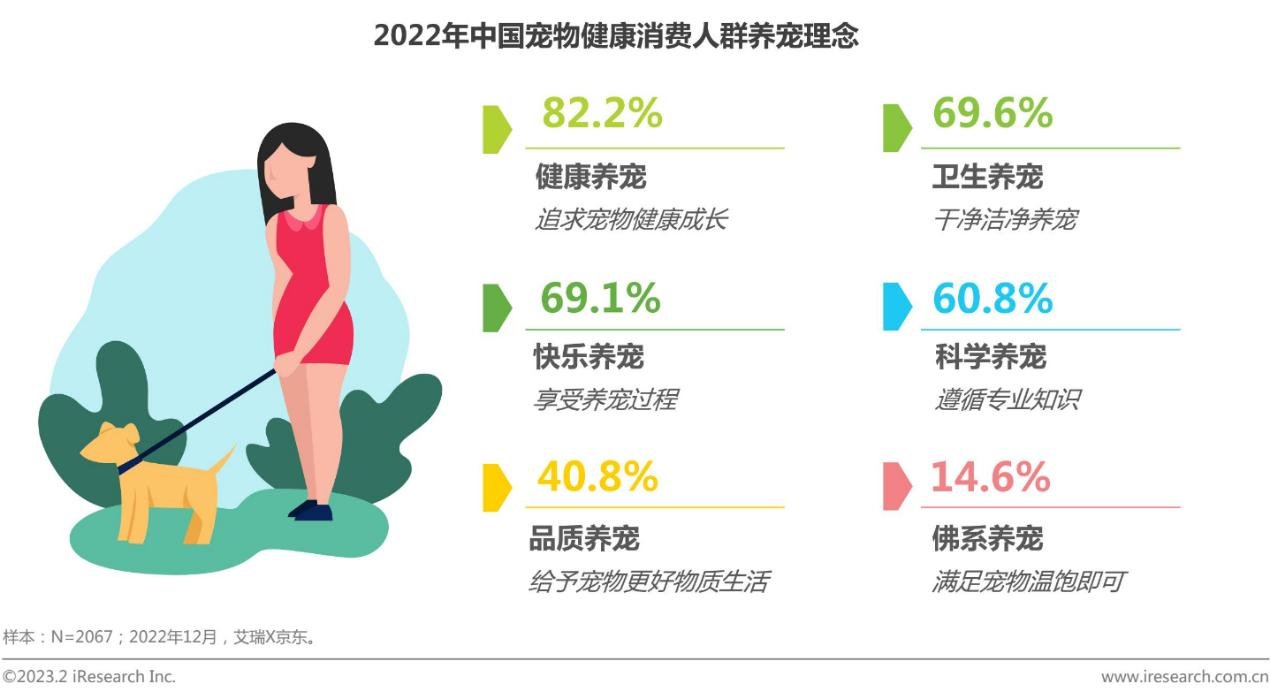
\includegraphics[scale=1]{CrowdPetConcept.jpg}
 	\caption{2022年中国宠物健康消费人群养宠理念}
 	\label{CrowdPetConcept}
	\end{figure}

\end{enumerate}

\paragraph{痛点分析}

尽管市场需求强劲,但现有的宠物服务平台大多存在以下问题:

\begin{itemize}
    \item \textbf{功能单一}:许多现有平台仅专注于某一领域,如宠物领养、社区互动或宠物新闻。这种缺乏整合性的服务让用户在使用过程中不得不频繁切换不同的平台,既不方便也降低了用户的整体体验。例如,用户可能需要在一个平台上查找宠物资讯,再去另一个平台参与社区讨论,导致使用体验断裂。
    \item \textbf{互动性差}:现有的宠物社区通常存在互动性不足的问题,导致社区氛围冷清,用户积极性不高。许多平台的评论和互动功能设计过于基础,用户发布内容后常常得不到及时的反馈,社区互动显得单调乏味。例如,一些平台的评论区缺乏实时通知和互动提醒,导致用户无法快速获得回应,进而影响他们的参与意愿和活跃度。
    \item \textbf{信息不对称}:用户在寻找宠物相关信息时,通常需要在多个网站或应用之间来回切换,信息分散且难以验证。例如,用户在为宠物寻找健康建议或训练方法时,往往会遇到信息来源不一致或不够权威的情况,导致决策困难。
    \item \textbf{缺少大语言模型}:现有的宠物服务平台很少利用大语言模型来提供个性化的用户体验,因此往往无法提供定制化的建议和支持。用户在寻求针对宠物特定行为、健康问题或护理建议时,常常会得到通用的、非针对性的回答。大语言模型的缺失使得现有平台在提供精确、个性化服务方面显得不足,导致用户体验降低。
    \item \textbf{用户交互性差}:用户交互性差会影响用户对平台的信任度和满意度。尽管一些平台在视觉设计上花费了大量的精力,但它们往往忽视了用户体验设计中的交互性元素。这意味着用户在浏览网站时可能会遇到操作不便或难以找到所需功能的问题。
\end{itemize}

\subsubsection{竞争分析}

\paragraph{市场上的类似产品}

当前市场上存在多种宠物服务平台,它们在特定领域内具有一定的用户基础,主要涵盖以下几类:

\begin{enumerate}
    \item \textbf{宠物领养平台}:这类平台专注于宠物领养信息的展示,通常提供详细的宠物资料、领养流程介绍等功能,帮助用户找到合适的宠物。如Petfinder和Adopt-a-Pet.com,前者是一个知名的在线宠物领养平台,拥有大量的宠物资料和收容所信息,后者侧重于提供一个全国性的宠物领养网络。但这些平台功能相对单一,往往仅限于信息展示,缺乏其他与宠物相关的服务,如宠物知识库或社交功能。
    \item \textbf{宠物百科平台}:此类平台以提供宠物知识为主,涵盖宠物种类、饲养方法、健康护理等内容。PetMD提供了一个综合性的宠物健康指南,用户可以在这里查找有关宠物健康的常见问题及解决方案;Vetstreet专注于提供专业的宠物健康和营养建议。虽然在信息资源方面表现优异,但通常缺乏互动性,用户难以就具体问题寻求即时帮助或与他人分享养宠心得。
    \item \textbf{宠物社区论坛}:社区论坛类平台为宠物爱好者提供了一个交流分享的场所,用户可以在平台上讨论养宠心得、分享宠物照片、或者求助问题。Reddit的r/pets子版块聚集了大量的宠物爱好者,用户可以在此自由发表看法;Pet Forums则是一个专门为宠物主人设计的论坛,用户可以在这里交流养宠经验。尽管社区氛围良好,但其功能大多停留在社交互动层面,缺少专业的知识支持或智能化服务,用户需要依赖其他渠道获取具体信息。
    \item \textbf{宠物新闻与资讯平台}:这类平台专注于宠物行业新闻、政策资讯和流行趋势报道,提供及时的行业动态信息。Pet360提供了关于宠物护理和训练的文章,以及最新的宠物产品和服务信息;PetNewsDaily.com以其专业的宠物护理文章和最新的宠物产品评测而闻名,提供最新的宠物护理技巧、行业新闻和产品评测等内容。然而,它们通常缺乏互动性和社交功能,用户获取信息后无法进一步讨论或分享。
\end{enumerate}

\paragraph{竞争优势}

“宠悦PetJoy” 作为一个综合性的宠物服务平台,相较于市场上现有的单一功能平台,具备以下显著的竞争优势:

\begin{enumerate}
    \item \textbf{多功能整合性}:

    与市场上大多数仅专注于单一功能的竞争平台不同,“宠悦PetJoy” 将宠物领养信息展示、宠物百科、宠物社区互动、宠物新闻和宠物AI助理等多种服务无缝整合在一个平台上。用户可以在一个平台内完成从信息获取到互动交流的所有需求,避免了跨平台操作的不便,显著提升了使用的便捷性。“宠悦PetJoy” 的多功能集成则提供了一站式服务,更好地满足了用户的多元化需求。

    \item \textbf{卓越的用户体验与交互设计}:

    PetJoy 致力于提供一个全面且以用户为中心的互动社区,凭借出色的用户交互设计和界面美观度,为用户带来独特的使用体验。平台不仅整合了丰富的宠物信息,且通过直观、易于操作的界面设计,使用户能够轻松导航和获取所需内容。我们特别考虑了不同人群的用户需求,确保界面的无障碍设计和友好的互动体验,以适应各种用户群体。

    从人机交互的角度来看,我们采用了响应式设计和动态反馈机制,使用户在社区互动中能够获得即时的视觉和操作反馈。这种设计不仅提升了用户的操作流畅性,还增强了平台的互动氛围。用户可以通过平台的社区功能,与其他宠物爱好者进行深度交流和互动,参与讨论,分享经验,从而建立一个积极而充满活力的社区环境。

    同时,平台的宠物AI助理通过自然语言处理技术,提供即时的宠物相关问题解答。这种智能化的支持不仅满足了用户在养宠过程中的即时需求,还通过个性化的互动增强了用户的整体体验。综合考虑用户交互设计和社区互动,“宠悦PetJoy”大幅提升了用户的满意度和平台的实用性。

    \item \textbf{信息可信度与透明度}:

    在宠物领养信息展示方面,用户最关心的是信息的可信度和透明度。许多宠物领养平台如PetAdoptionNetwork.org规模较小,信息更新不够频繁,最新的更新时间仅在2022年,没有足够的资源来实施严格的信息审核程序。

    “宠悦PetJoy” 平台提供了经过审核的领养信息,确保用户在浏览和选择领养宠物时能够获得真实、可靠的资料。这种透明的信息展示方式,提高了用户对平台的信任感。

    \item \textbf{技术支持的服务}:

    虽然市场上的一些平台在特定领域内(如信息展示或社交互动)有着较高的专业性,但在智能化服务方面往往不足。如Pet Forums、Reddit的r/pets子版块相比,虽然这些社区提供了丰富的用户生成内容,但缺乏即时性和专业知识。

    “宠悦PetJoy” 通过引入宠物AI助理,提供即时的宠物问题解答和建议服务,使用户能够更快、更便捷地获得所需信息。这一技术支持的服务不仅提升了用户体验,还为用户在实际的宠物管理和照顾过程中提供了额外的帮助。

\end{enumerate}

\paragraph{差异化特点}

“宠悦PetJoy”在竞争激烈的市场中,通过以下差异化特点建立了其独特的市场定位:

\begin{enumerate}
    \item \textbf{全方位的多功能平台}:相比于市场上那些专注于单一功能的竞争平台,如Pet360,这些平台虽然提供宠物新闻和资讯,但缺乏社区互动和即时问答功能。宠悦提供了一个多功能一体化的平台,集宠物领养信息、百科知识、社区互动、新闻资讯、以及宠物AI助理服务于一身。用户在平台内即可完成从获取知识到互动交流的所有需求,无需频繁切换至其他平台。
    
    \item \textbf{即时问题解答服务}:通过宠物AI助理,用户可以在平台上获得即时的宠物相关问题解答和建议,这一功能是许多市场上的平台所缺乏的。这些平台如PetMD,虽然提供丰富的宠物健康信息,但缺乏即时交互能力。宠悦的宠物AI助理为用户提供了一个便捷的互动工具,使他们在遇到问题时能够快速获得支持。
    
    \item \textbf{增强的社交互动}:其他宠物平台如PetConnectForum.com提供了一个活跃的社区,但其功能较为传统,主要依靠帖子和评论来互动。除了提供丰富的宠物信息外,宠悦还通过社区功能增强了用户之间的互动。相比于其他信息展示为主的平台,我们的社区功能使用户能够更深入地参与到宠物爱好者的交流和分享中,增强了用户的参与感和归属感。
    
    \item \textbf{信息审核与透明度}:由于其非营利性质,平台如RescueMe.org,更侧重于救助活动而非信息审核。在宠物领养信息展示方面,PetJoy通过严格的审核机制,确保平台上的信息真实可靠。这种信息的透明度不仅为用户提供了保障,也提高了平台的可信度,进一步巩固了其市场竞争力。
\end{enumerate}

\subsubsection{项目目标}

\paragraph{功能目标}

宠悦的功能目标是提升平台的核心服务质量和用户体验,通过明确的功能实现,确保每个模块的目标能够满足用户需求和平台运营要求。具体目标包括:

\begin{itemize}
    \item \textbf{实现用户和通知模块}:
    \begin{itemize}
        \item \textbf{完善用户信息管理}:提供用户友好的界面,允许用户便捷地更新个人信息(如头像、昵称、性别、生日等),并设置隐私选项。确保用户信息的安全存储,并根据用户选择灵活管理隐私设置。 
        \item \textbf{高效的通知系统}:实现一个实时通知机制,向用户推送互动消息等,以帮助用户及时了解与其他用户的互动情况和平台的重要信息。设计直观的通知界面,使用户能够方便地查看和管理收到的通知,
    \end{itemize}

    \item \textbf{实现宠物社区模块}:
    \begin{itemize}
        \item \textbf{帖子发布和互动}:支持用户发布带有宠物照片和文字的帖子,并提供编辑和删除功能。实现点赞、评论和收藏功能,增强用户对帖子内容的互动性,并通过数据统计分析帖子受欢迎程度。通过帖子分类功能组织内容,帮助用户更快找到感兴趣的帖子。        
        \item \textbf{社区互动优化}:提供评论功能,允许用户对帖子进行详细评论,并支持评论的点赞和回复,促进讨论的深度。设计用户友好的界面,确保用户在参与社区互动时的操作便捷,提升用户的使用体验。
    \end{itemize}

    \item \textbf{实现宠物新闻模块}:
    \begin{itemize}
        \item \textbf{新闻发布和管理}:建立新闻发布系统,允许管理员发布和更新宠物相关新闻,涵盖宠物健康、护理等多个领域。通过新闻标签功能,用户可以根据兴趣筛选新闻内容,提高新闻的可发现性。提供新闻详情页,展示完整的新闻内容、发布时间等信息,并支持用户对新闻进行评论和反馈。
        \item \textbf{用户互动和反馈}:实现点赞和点踩功能,允许用户对新闻内容进行评价,提供对新闻内容的快速反馈。提供评论功能,用户可以在新闻下方发表评论,分享自己的看法和经验。设计直观的新闻界面,确保用户能够方便地浏览和阅读新闻,提升用户的阅读体验。
    \end{itemize}

    \item \textbf{实现宠物领养模块}:
    \begin{itemize}
            \item \textbf{宠物信息展示}:提供详细的宠物信息展示,包括名称、年龄、品种、健康状况、位置和领养状态等,帮助用户了解每只宠物的基本情况。记录特殊护理需求和饮食习惯等详细信息,以便有意领养的用户能够了解宠物的具体需求。
            \item \textbf{用户界面设计}:每只宠物将以信息卡片的形式展示,卡片包括宠物的基本信息(名称、年龄、品种)、健康状况、位置、领养状态以及其他相关细节。在宠物信息卡片上添加“查看详情”按钮,用户点击后将进入宠物的详细信息页面。该页面将展示更全面的宠物资料,包括高分辨率的照片、详细的护理需求、饮食习惯、性格描述等。
    \end{itemize}

    \item \textbf{实现宠物AI模块}:
    \begin{itemize}
            \item \textbf{智能服务提供}:引入人工智能技术,提供宠物行为解释、健康建议等智能服务。用户可以输入宠物相关信息或问题,AI 助理基于大数据提供个性化的评估和建议。设计简洁的用户界面,确保用户能够方便地与 AI 助理进行互动,输入问题并获取反馈。 
            \item \textbf{用户交互优化}:提供友好的交互体验,确保用户能够轻松使用AI助理的功能,提升整体用户体验。设计直观的问答界面,使用户能够方便地输入问题或请求,并获得快速、准确的回答。
    \end{itemize}
\end{itemize}

\paragraph{功能实现方案}

为了实现“宠悦PetJoy”的功能目标,我们将采取以下措施:

\begin{enumerate}
    \item \textbf{用户和通知模块}:设计一个用户信息管理界面,允许用户更新个人信息并设置隐私选项。实现实时通知系统,向用户推送互动消息,并提供简洁的通知管理界面。

    \item \textbf{宠物社区模块}:开发支持用户发布宠物帖子的功能,包括照片、文字、点赞、评论和收藏。帖子将按分类组织,用户可以通过评论和互动功能参与讨论。

    \item \textbf{宠物新闻模块}:建立新闻发布系统,允许管理员发布和更新宠物相关新闻。用户可以根据新闻标签筛选内容,进行点赞、评论和反馈。

    \item \textbf{宠物领养模块}:以信息卡片形式展示宠物信息,包括名称、年龄、健康状况等。用户可以查看详细资料,了解特殊护理需求,并通过筛选功能查找适合的宠物。

    \item \textbf{宠物AI模块}:引入AI技术,为用户提供宠物行为和健康建议。设计直观的问答界面,支持自然语言输入,确保用户能够获得准确的反馈。
\end{enumerate}

\subsubsection{相关方和利益关系}

“宠悦PetJoy”平台的成功运营离不开各相关方的参与和支持,包括:

\begin{itemize}
    \item \textbf{用户}:宠物爱好者是平台的核心用户群体,他们通过平台获取信息、分享经验、参与社区互动,并获得实际的宠物服务。用户的参与和活跃度是平台成功的关键。
    
    \item \textbf{合作伙伴}:平台将与宠物用品商家、宠物医院、动物收养中心等建立合作伙伴关系,共同为用户提供高质量的产品和服务。合作伙伴的资源和服务将极大地丰富平台的内容和功能,提升用户的整体体验。
    
    \item \textbf{内部团队}:包括平台的开发、运营、市场推广团队。开发团队负责平台的技术实现和维护,确保系统的稳定性和功能的持续更新;运营和推广团队则通过各种市场活动和策略,扩大平台的用户基础,提高品牌知名度。
    
    \item \textbf{政府}:政府部门是平台运营中的重要支持者,通过制定和监督相关的法规政策,为平台提供行业指导和支持。政府的支持有助于确保平台的合规运营,并推动宠物行业的健康发展。

    \item \textbf{社会}:社会组织和公众对宠物福利和动物保护的关注也是平台运营中的重要因素。通过与社会组织的合作,平台可以开展公益活动,提升社会责任感,并增强公众对平台的信任和支持。

\end{itemize}

各相关方在平台的运营中相互依存,共同推动平台的发展。用户的参与带动平台的流量和活跃度,合作伙伴的资源和服务丰富了平台的内容,内部团队则通过技术和运营手段保障平台的稳定性和持续改进。政府和社会的支持则为平台提供了规范和公益的支持,促进了平台的长期发展。

\subsection{系统功能概述}

\subsubsection{用户与通知模块}

\paragraph{用户管理}

在这部分,我们将从注册与登录机制、个人信息维护、用户角色与状态管理、以及隐私偏好设置等四个关键方面,规划和设计用户管理功能的整体架构与安全策略,确保用户能够便捷、安全地访问系统,同时提供个性化体验和多层次的隐私与权限管理。

\begin{itemize}
	\item \textbf{注册与登录机制}:用户管理功能的核心是确保用户能够安全便捷地访问系统。系统采用手机号注册与登录的机制,用户通过验证手机号码来创建账号并登录平台。系统支持短信验证码方式提升密码安全性。
	\item \textbf{个人信息维护}:系统允许用户随时编辑和更新个人信息,包括用户名、个人简介、联系方式、头像链接、性别和出生日期等。用户能够根据自己的需求,个性化自己的个人资料,提升使用体验。个人信息的编辑界面友好且易于操作,同时系统会确保用户隐私的安全性。
	\item \textbf{用户角色与状态管理}:系统支持多种用户角色的管理,例如普通用户、管理员等,不同角色有不同的权限设置。管理员可以通过后台管理界面对用户的状态进行控制,包括激活和禁用用户账号。角色与状态管理功能确保系统能够满足不同类型用户的使用需求,并且通过权限控制来维护系统的安全和秩序。
	\item \textbf{隐私偏好设置}:在个性化设置功能中,用户可以自主控制个人信息的公开范围,以保障隐私安全。用户能够选择哪些信息可以公开显示,哪些信息仅对自己可见。这包括但不限于电话号码、性别、出生日期等敏感信息的公开与隐藏设置。系统提供了灵活的隐私控制选项,以满足用户对隐私保护的需求,确保用户可以安心使用平台。
\end{itemize}

\paragraph{用户互动}

在这部分,我们将从打卡记录功能、关注与粉丝管理、以及用户留言功能三个方面,规划和设计用户互动模块,确保通过日常互动、社交网络的建立,以及多样化的交流方式,来提升平台的用户参与度和粘性。

\begin{itemize}
	\item \textbf{打卡记录功能}:用户互动中的打卡记录功能支持用户每日记录与宠物的互动活动。这一功能旨在鼓励用户持续参与平台,培养与宠物互动的习惯,并通过每日打卡来展示用户的活跃度。用户可以查看自己的打卡历史,并获得平台的激励或奖励,增强平台的用户粘性。
	\item \textbf{关注与粉丝管理功能}:平台提供用户之间的关注功能,用户可以关注其他用户,形成粉丝关系。这一功能增强了平台的社交互动性,使用户可以轻松获取自己关注的用户的动态和更新。通过关注功能,用户可以建立更紧密的社交网络,增加与其他用户的互动频率。
	\item \textbf{用户留言功能}:用户留言功能允许用户通过留言的方式进行沟通,增加平台的互动性与用户粘性。用户可以在其他用户的主页或动态下留言,表达意见、建议或互动。这一功能使用户能够在平台内建立更加活跃和多样的交流方式,提升用户体验和平台的社交属性。
\end{itemize}

\paragraph{通知系统}

在这部分,我们将从通知的接收与发送、通知分类与状态跟踪两个方面,规划通知系统的功能设计,确保在开发过程中能够通过及时传达信息和有效管理通知分类,来提升用户的参与度与互动性,并帮助用户更好地管理和跟踪重要信息。

\begin{itemize}
	\item \textbf{通知的接收与发送}:通知系统支持用户接收和发送通知,以确保重要信息能够及时传达给用户。用户可以接收来自系统或其他用户的通知,这些通知可以包括新的关注者、评论、回复、平台更新等内容。通过这一功能,平台可以提升用户的参与度和互动性,同时帮助用户更好地管理和跟踪他们的社交活动。
	\item \textbf{通知分类与状态跟踪}:为了便于管理和使用,通知系统支持将通知分类为系统通知和个人通知。系统通知通常涉及平台更新、系统公告等,而个人通知则包括用户间的互动信息,如新的评论或关注。用户可以通过查看通知的已读状态来跟踪自己是否已处理某条通知,避免遗漏重要信息。这一功能不仅提高了通知的可管理性,还增强了用户对平台的使用体验。
\end{itemize}

\paragraph{用户安全性需求}

在这部分,我们将从重置密码、修改绑定手机号、以及注销账号三个方面,规划和设计用户安全性需求模块,提供用户自主可控的安全保障,维护用户的隐私权和数据安全。

\begin{itemize}
	\item \textbf{重置密码}:平台提供安全的密码重置功能,帮助用户在忘记密码或怀疑账号安全受到威胁时,迅速恢复账号访问权限。用户通过提供绑定的手机号等方式,验证信息以完成密码重置过程。此功能确保用户能够在安全的环境中重新设置密码,保障账号的安全性。
	\item \textbf{修改绑定手机号}:用户可以通过平台安全地更新绑定的手机号码,确保他们的联系信息始终是最新的。平台会对用户的更改请求进行验证,例如通过短信验证码的方式,确认新手机号的有效性。这一功能保证了用户的个人信息准确性,方便平台在需要时联系用户。
	\item \textbf{注销账号}:平台支持用户在需要时安全地注销账号。用户可以在平台设置中发起注销请求,经过多步确认以避免误操作。注销账号后,用户的个人数据将被删除,确保用户数据的自主可控性,并符合相关的数据保护法规。此功能为用户提供了退出平台的自主权,并在保证数据安全的前提下,满足了用户的隐私需求。
\end{itemize}

\subsubsection{宠物社区模块}

\paragraph{帖子发布与管理}

在这部分,我们将从帖子发布与分类、帖子置顶功能、以及图片上传功能三个方面,规划和设计帖子发布与管理模块,提升用户体验,优化内容组织,并增加用户的互动和参与度。

\begin{itemize}
	\item \textbf{帖子发布与分类}:用户可以通过平台发布与宠物相关的内容,并为帖子选择合适的分类标签。帖子分类的设计旨在提升信息检索效率,使用户能够快速找到自己感兴趣的内容。通过这种分类机制,平台能够组织和管理大量的用户内容。
	\item \textbf{帖子置顶功能}:为了保证优质内容的曝光度,平台管理员可以将重要帖子置顶。被置顶的帖子会在相关页面的显著位置展示,确保这些内容能够获得更多的阅读和互动。通过帖子置顶功能,平台能够引导用户关注有价值的内容,提高社区内容的质量和用户参与度。
	\item \textbf{图片上传功能}:平台支持用户在发布帖子时上传宠物图片,使内容更加生动和吸引人。图片上传功能不仅丰富了帖子内容的表现形式,还为用户提供了展示宠物的途径,增强了用户的互动体验。
\end{itemize}

\paragraph{帖子互动}

在这部分,我们将从评论功能、点赞点踩功能、举报功能以及收藏功能四个方面,规划和设计帖子互动模块,确保平台能够通过多层次的对话、直观的内容反馈机制,以及有效的社区管理,用户能够方便地保存和访问感兴趣的内容,提升用户交流体验,同时维护社区的健康环境,增强用户的参与感。

\begin{itemize}
	\item \textbf{评论功能}:平台为用户提供了评论和回复功能,使得用户可以在帖子下发表自己的看法,并与其他用户进行互动。通过这种方式,用户能够在平台上展开深度交流,分享经验和见解,增强社区的互动性和参与感。评论功能支持层级结构,用户可以直接回复他人的评论,从而形成多层次的对话,提高讨论的深度和广度。
	\item \textbf{点赞点踩功能}:用户可以通过点赞或点踩功能,表达对帖子和评论的喜好或不满。这种简单而直接的互动方式,有助于内容创作者了解其内容的受欢迎程度,提升用户体验感。
	\item \textbf{举报功能}:为了维护社区的健康和谐,平台为用户提供了举报功能。用户可以举报不当或违反社区规范的内容,平台运营团队将根据举报信息及时采取措施,如删除违规内容或对违规用户进行处罚。举报功能确保了社区环境的安全性和规范性,提升了用户对平台的信任感。
	\item \textbf{收藏功能}:用户可收藏感兴趣的帖子,方便后续查阅。收藏功能让用户可以轻松访问之前保存的内容,内容创作者也能通过收藏数据获取用户反馈,进一步提升内容的质量和吸引力。
\end{itemize}

\subsubsection{宠物新闻模块}

\paragraph{新闻发布与管理}

在这部分。我们将从新闻分类功能、新闻置顶功能、以及图片及视频管理功能三个方面,规划和设计新闻发布与管理模块,确保用户能够方便地查找和浏览感兴趣的新闻,通过置顶功能突出重要新闻,并利用多媒体资源增强新闻的视觉吸引力,从而提升新闻的可访问性、曝光度和用户阅读体验。

\begin{itemize}
	\item \textbf{新闻分类功能}:新闻分类功能通过对新闻内容进行系统化的分类,使得用户能够更加方便地查找和浏览自己感兴趣的内容。平台为每篇新闻分配标签,利用灵活的标签系统来组织新闻内容。这不仅提升了新闻的可访问性,还帮助用户在广泛的内容中快速找到符合其兴趣的新闻。
	\item \textbf{新闻置顶功能}:重要新闻或平台特别推荐的内容可以通过置顶功能优先显示在新闻页面的顶部,确保这些关键信息能够引起用户的关注。置顶功能的实现基于新闻表中的置顶字段,管理员可以通过设置此字段来控制新闻的展示顺序。这种机制不仅能够提升重要内容的曝光度,还能增加用户对平台资讯的信任和依赖。
	\item \textbf{图片及视频管理功能}:每篇新闻都可以配有相应的图片或视频,以增强新闻的视觉吸引力。新闻表中存储了封面图片链接字段,用于展示新闻的主要视觉元素。此外,新闻内容中可以嵌入多媒体资源,这不仅丰富了新闻的表现形式,还能够更好地吸引用户的注意力。通过图文并茂的新闻内容,平台能够提供更加生动和有吸引力的阅读体验,提升用户的阅读参与度。
\end{itemize}

\paragraph{新闻互动}

在这部分,我们将从评论功能、点赞点踩功能、举报功能以及收藏功能四个方面,规划和设计新闻互动模块,确保用户能够通过评论与其他用户互动,收藏感兴趣的新闻内容,表达对新闻内容的意见,并通过点赞、点踩和举报功能直接反馈内容质量,帮助平台维护社区秩序,提升平台内容的整体质量。

\begin{itemize}
	\item \textbf{评论功能}:用户可以通过评论功能对新闻内容进行反馈和讨论,增强新闻内容的互动性和社区的参与感。评论区不仅是用户表达观点的平台,还可以成为信息交流和思维碰撞的场所。通过评论,用户可以更深入地讨论新闻内容,提出自己的见解,或与其他用户进行互动,形成丰富的讨论氛围。
	\item \textbf{点赞点踩功能}:用户可以通过点赞或点踩功能对新闻内容和评论进行快速的反馈,反映他们对内容的认可或质疑。这一功能帮助平台识别受欢迎的新闻,点赞数的增加通常代表内容质量的提升,而点踩数的上升则可能提示内容需要改进。这种互动机制不仅鼓励优质新闻的生产,也为用户提供了一个直接表达意见的渠道。
	\item \textbf{举报功能}:用户可以使用举报功能来标记不当或不适合的评论,帮助平台维护内容的健康和社区的秩序。举报机制是确保平台内容符合社区规范的重要手段。通过对举报内容的及时处理,平台可以迅速应对和纠正违反规定的行为,保证社区环境的安全和友好。同时,举报功能还激励用户积极参与社区管理,共同维护良好的社区氛围。
	\item \textbf{收藏功能}:新闻收藏功能为用户提供了一种快速保存感兴趣内容的方式,方便日后随时查看。这一功能增加了用户在平台上的参与感,通过一键收藏,用户可以将任何感兴趣的新闻内容保存到他们的个人收藏列表中,无需担心日后找不到相关内容。对于不再感兴趣的新闻,用户可以轻松将其从收藏列表中删除,确保收藏内容的时效性和相关性。这一功能极大地提升了用户的阅读体验,使得新闻平台成为用户日常获取信息的首选渠道。
\end{itemize}

\subsubsection{宠物领养模块}

\paragraph{宠物信息发布}

在这部分,我们将从宠物基本信息展示、健康状况记录、以及特殊需求说明三个方面,规划和设计宠物信息发布模块,确保潜在领养者能够全面了解宠物的基本情况和健康状况,并提前知晓宠物的特殊需求,提升了平台在宠物领养过程中的专业性和可信度。

\begin{itemize}
	\item \textbf{宠物基本信息展示}:宠物信息发布功能旨在向潜在领养者展示宠物的详细信息,帮助他们了解每只宠物的基本情况。在这个模块中,平台会展示宠物的名称、年龄、品种以及宠物的照片等基本信息。通过直观的信息展示,用户能够快速浏览和筛选出感兴趣的宠物。这些基本信息不仅为潜在领养者提供了直观的认识,还能帮助他们根据个人喜好和生活条件选择最适合的宠物。此外,宠物的年龄和品种等信息帮助用户初步了解宠物的特点,进一步助力用户做出领养决策。
	\item \textbf{健康状况记录}:为了确保领养过程的透明性和规范性,平台详细记录并展示每只宠物的健康状况。这一功能让潜在领养者了解宠物的健康历史、当前健康状态以及疫苗接种情况。健康状况的透明化展示不仅帮助领养者做好准备,也能有效减少领养后可能遇到的健康问题。同时,通过健康状况的详细记录,平台也能够更好地管理和追踪宠物的健康数据,确保每只宠物在等待领养期间都能得到充分的医疗照顾。
	\item \textbf{特殊需求说明}:为了帮助潜在领养者充分了解每只宠物的独特需求,平台还提供了宠物的特殊需求说明。这些需求可能包括饮食习惯、特殊护理要求、性格行为特征等。通过明确的特殊需求说明,领养者能够提前了解宠物在日常生活中的特殊需求,确保他们具备必要的条件来照顾宠物。
\end{itemize}

\paragraph{领养流程管理}

在这部分,我们将从领养申请帮助和领养状态跟踪两个方面设计领养流程管理模块,确保用户了解领养要求,并通过透明的合同条款和实时状态更新,提升领养过程的规范性和透明度。

\begin{itemize}
	\item \textbf{领养申请帮助}:系统将向用户提供详细的领养注意事项,帮助用户了解领养宠物的基本要求和注意事项。系统会列出宠物领养的基本条件,这些条件将帮助用户自我评估是否符合领养要求,避免因不符合条件而影响领养成功率。用户可以在线浏览宠物领养合同的示例,合同中详细列出了领养条款、责任和义务。用户需要仔细阅读并同意合同条款,确保双方权益的明确和保护。领养合同的透明化设计可以增加领养过程的规范性和双方的信任感。
	\item \textbf{领养状态跟踪}:领养状态跟踪功能为用户提供了实时更新宠物领养进度的服务。用户可以通过系统查看到申请的宠物当前的领养状态,如“待领养”或 “已领养”,方便用户了解领养进展。
\end{itemize}

\subsubsection{宠物百科模块}

\paragraph{品种介绍}

在这部分,我们将从品种特性描述和品种分类信息两个方面设计品种介绍模块,确保用户能够通过详细的特性描述和系统化的分类,快速了解不同宠物品种的独特特性和养护需求。

\begin{itemize}
	\item \textbf{品种特性描述}:品种特性描述功能提供了详细的宠物品种信息,帮助用户了解不同宠物品种的独特特性和养护需求。这一功能包括对各个宠物品种的详细介绍,例如起源地、体型、毛色、寿命、性格特征和饮食习惯等。每种宠物品种的介绍将包括相关图片,帮助用户更直观地了解宠物的外观和特点。通过详细的特性描述,用户能够做出更加明智的选择,确保选择的宠物符合他们的生活方式和个人偏好。
	\item \textbf{品种分类信息}:品种分类信息功能通过系统化的分类结构,提供清晰的宠物品种分类,帮助用户快速找到他们感兴趣的宠物品种。系统将宠物品种分为不同的类别和子类,每个类别和子类都有具体的信息和详细描述。特别的是,平台还提供了可视化的起源地地图,直观展示各品种的历史渊源和地理分布。通过这些增强的分类和描述,平台能够提供高质量的宠物百科内容,提升用户的满意度,增加平台的专业性。
\end{itemize}

\paragraph{护理指导}

在这部分,我们将从行为训练指导和健康护理知识两个方面设计护理指导模块,确保用户能够通过科学的训练技巧和全面的健康管理信息,有效培养宠物的良好行为习惯,并提升宠物的健康和生活质量。

\begin{itemize}
	\item \textbf{行为训练指导}:行为训练指导功能提供科学的宠物训练技巧,帮助用户培养宠物的良好行为习惯。这些训练技巧通过详细的步骤说明和实际案例,帮助用户更好地理解和应用,提高训练的成功率。用户可以根据宠物的不同需求和个性,选择合适的训练方法,培养宠物的良好行为习惯。
	\item \textbf{健康护理知识}:健康护理知识功能提供全面的宠物健康管理信息,帮助用户更好地照顾宠物的健康。通过详细的护理指导和健康建议,用户能够更科学地管理宠物的健康和日常生活,提升宠物的生活质量和幸福感。同时,平台还将根据用户的反馈和需求,定期更新和优化护理指导内容,确保信息的时效性和实用性。
\end{itemize}

\subsubsection{宠物护理模块}

\paragraph{视频播放}

在这一部分,我们将从宠物护理视频的播放和观看体验两方面设计视频播放功能,确保用户能够通过高质量的视频内容,学习到科学有效的宠物护理技巧,并根据自己的需求进行播放控制。

\begin{itemize}
	\item \textbf{宠物护理视频播放}:该功能旨在为用户提供宠物护理相关的视频,涵盖了宠物健康管理、饮食营养、清洁美容等不同方面。用户可以从不同的视频中选择感兴趣的内容进行观看,学习科学的宠物护理方法。每个视频都会有相应的描述,帮助用户提前了解视频内容,方便选择合适的护理知识进行学习。
	\item \textbf{观看体验提升}:用户可以在视频播放过程中通过操作控制栏调整播放进度、音量以及切换全屏或缩放模式,提升观看体验。此外,用户还可以根据自己的需求调整视频的播放速度,以更好地理解和应用视频中的宠物护理技巧。平台为用户提供了灵活的观看选项,确保不同用户的个性化需求都能得到满足。
\end{itemize}

\paragraph{视频下载}

在这一部分,我们将设计视频下载功能,确保用户能够保存感兴趣的宠物护理视频,便于随时回看和离线观看。

\begin{itemize}
	\item \textbf{宠物护理视频下载}:用户可以将平台上的宠物护理视频下载到本地进行保存。该功能帮助用户在没有网络的情况下也能随时回看重要的视频内容,掌握更多的宠物护理知识。视频的下载操作简单快捷,确保用户在离线时也能获得高质量的学习体验。
\end{itemize}

\subsubsection{宠物AI模块}

宠物AI模块利用先进的人工智能技术,为用户提供个性化的宠物护理建议。这些建议基于宠物的具体信息,如品种、年龄、健康状况等,为用户提供定制化的护理方案。宠物AI模块不仅提升了用户的宠物护理能力,还增强了平台的互动性和趣味性,吸引用户更频繁地使用系统。

\subsection{用户特点部分}

\subsubsection{用户群体分析}

\paragraph{目标用户}

我们的目标用户主要有宠物爱好者、宠物新手、专业饲养员与宠物医生和宠物领养关注者这几类群体。

\begin{itemize}
	\item \textbf{宠物爱好者}:在“宠悦”平台的设计初期,我们就预计宠物爱好者将成为该平台的主要用户群体。这些用户通常已经拥有宠物,并对宠物的养护、训练、饮食等方面有一定的经验。我们设想,这部分用户将热衷于在“宠物社区”功能中分享他们的日常经历,发布宠物的照片和视频,与其他宠物主人进行互动和讨论。为了满足他们的需求,我们计划设计一个简洁易用的界面,支持多种互动方式,如点赞、评论和分享。
	\item \textbf{宠物新手}:在我们的预期中“宠悦”将吸引大量首次养宠物的用户。这些新手用户可能对宠物的日常照料缺乏经验,急需获得相关知识和帮助。我们设想,“宠物百科”功能将为他们提供详尽的宠物护理指南和常见问题解答。此外,“宠物AI”功能预计将帮助他们解决日常遇到的具体问题,如宠物健康、训练技巧等。为了更好地服务这部分用户,我们将考虑提供简单明了的导航栏,以便他们能够快速找到所需信息。
	\item \textbf{专业饲养员与宠物医生}:在我们的规划中,专业饲养员和宠物医生将是社区内的重要用户群体。这些用户拥有深厚的专业知识和丰富的实践经验,我们期望他们在社区中扮演知识传授者的角色,定期分享专业的养护经验和治疗建议。社区的发帖与评论功能预计将为他们提供一个与普通用户直接互动的平台,解答他们的疑问并提供专业建议,这有助于吸引和留住这些高价值用户。
	\item\textbf{宠物领养关注者}:我们预计宠物领养将成为“宠悦”社区的一个重要功能板块,吸引那些希望领养宠物的用户。这些用户可能是个体,也可能是动物保护组织或宠物救助机构。在我们的设想中,他们将主要使用“宠物领养”功能,浏览待领养宠物的信息,查看相关领养合同和注意事项,甚至发布领养信息。为了支持他们的需求,我们计划提供一个全面的领养信息管理系统,帮助他们方便快捷地找到合适的宠物,并完成领养流程。
\end{itemize}

\paragraph{用户分布}

下面我们将基于全球化用户来分析用户分布。鉴于“宠悦”将支持十种语言,我们预计用户群体将遍布全球各地。不论是中国、日本还是欧洲、美洲,不同地区、不同文化的宠物爱好者都可以在“宠悦”平台上找到自己的同伴。此外,不同地区的用户对界面和功能的偏好可能会有所差异,我们为此进行了亮暗模式的相关设计。

\paragraph{用户动机}

我们认为用户使用“宠悦”平台的主要动机有信息获取、社交互动和宠物领养。

\begin{itemize}
	\item \textbf{信息获取}:我们推测,“宠悦”的许多用户将以获取宠物相关的信息为主要动机。尤其是宠物新手,他们预计会频繁访问“宠物百科”以学习养宠技巧,并依赖“宠物AI”来获得快速且实用的解答。为了满足这一需求,我们计划整合大量优质的宠物知识内容,并确保信息的易读性和实用性。
	\item \textbf{社交互动}:我们预期,“宠物社区”将成为用户互动的主要场所。通过分享他们与宠物的日常生活,用户将能够与志同道合的人建立联系,获得情感上的支持和共鸣。我们设想,社区将提供丰富的互动功能,鼓励用户之间的交流与分享,进一步增强社区的凝聚力。
	\item \textbf{宠物领养}:对于有领养意愿的用户,我们预计“宠物领养”功能将成为他们关注的核心。他们将希望通过平台找到合适的宠物,并了解领养过程中的各项注意事项。为了使这一功能更具吸引力,我们计划提供详尽的宠物信息和透明的领养流程,并确保用户在领养过程中获得全面的指导和支持。
\end{itemize}

\subsubsection{用户行为分析}

\paragraph{活跃度分析}

下面我们将根据功能使用频率和用户互动习惯进行活跃度分析。

\begin{itemize}
	\item \textbf{功能使用频率}:在“宠悦”社区中,用户的活跃度预计将因功能的不同而有所差异。根据我们对用户需求的预判,“宠物社区”和“宠物AI”功能将成为用户最常访问的板块。我们预计,这些功能将吸引大量的日常活跃用户,特别是在工作日的晚上和周末的全天期间,用户的访问量可能会显著增加。
	\item \textbf{用户互动习惯}:我们预计,“宠悦”社区的用户将表现出较强的互动意愿。这些互动可能包括发布帖子、评论他人内容以及使用“宠物AI”功能获取信息。不同观点的用户之间的碰撞同样有助于加强用户之间的互动。
\end{itemize}

\paragraph{功能使用偏好}

这部分我们将分析用户对于宠物社区和宠物百科与AI功能的使用偏好。

\begin{itemize}
	\item \textbf{宠物社区}:在我们的预判中,宠物社区功能将受到资深宠物爱好者的青睐。这些用户可能会频繁发布关于宠物的生活点滴、健康建议和训练技巧的内容,同时也会积极参与其他用户的讨论和点赞行为。
	\item \textbf{宠物百科与AI}:对于宠物新手用户而言,我们预计“宠物百科”与“宠物AI”功能将是他们最常使用的工具。这些用户可能会在初次接触社区时,首先利用“宠物百科”查找基本的宠物护理知识,如饮食指南、疾病预防等。我们计划在“宠物AI”中嵌入智能问答系统,帮助新手用户快速找到具体问题的答案。
\end{itemize}

\paragraph{内容交互分析}

用户主要通过用户生成内容(UGC)和内容消费模式进行内容交互。

\begin{itemize}
	\item \textbf{用户生成内容(UGC)}:我们预期,社区的用户生成内容(UGC)将成为“宠悦”平台的核心资产。这些内容可能包括用户分享的宠物照片、护理心得、疾病治疗经验等。我们计划通过一系列的机制,如点赞、评论、收藏数排行和置顶,鼓励用户生成更多高质量的内容。同时,社区将设有内容审核机制,确保UGC的质量和真实性,以维护社区的良好氛围和用户的信任度。
	\item \textbf{内容消费模式}:根据我们的推测,用户在“宠悦”社区的内容消费模式将表现出明显的个性化特点。部分用户可能更倾向于阅读和浏览,而不是主动发布内容。为了满足这些用户的需求,我们计划在社区中提供丰富的内容浏览选项,如主题分类和热门推荐。考虑到用户的碎片化时间使用习惯,我们将设计一些短内容形式,让用户在短时间内获得有价值的信息。
\end{itemize}

\subsubsection{用户需求与反馈分析}

\paragraph{语言支持需求}

接下来我们将从多语言支持的重要性和用户反馈的预期来说明语言支持需求。

\begin{itemize}
	\item \textbf{多语言支持的重要性}:由于“宠悦”社区将支持十种语言,我们预计不同语言用户在使用平台时会有不同的需求和反馈。为了确保每位用户都能获得良好的体验,我们将重点关注各语言版本的准确性和用户友好性,尤其是在宠物相关术语的翻译上。我们计划通过用户反馈机制,持续改进各语言版本的内容,以满足全球用户的需求。
	\item \textbf{用户反馈的预期}:我们认为用户将对语言支持提出各种建议和意见,特别是在本地化翻译和文化适应性方面。为了有效处理这些反馈,我们将定期收集和分析用户反馈,并在社区更新中逐步实施改进措施。
\end{itemize}

\paragraph{用户体验反馈}

这一部分我们从亮暗模式的需求和界面设计与操作便捷性来分析用户体验反馈。

\begin{itemize}
	\item \textbf{亮暗模式的需求}:随着移动设备的普及和用户习惯的变化,我们预计亮暗模式将成为“宠悦”社区的重要功能。许多用户可能更倾向于在夜间使用暗模式,以减轻眼睛疲劳。为了提供最佳的用户体验,我们计划在亮暗模式之间提供无缝切换功能,并根据用户反馈进一步优化界面的视觉效果和颜色搭配。	
	\item \textbf{界面设计与操作便捷性}:我们推测用户将在社区界面的设计和操作便捷性方面提出大量反馈。用户可能会要求更直观的导航栏、更清晰的布局,以及更快速的响应时间。为了满足这些需求,我们将采取用户中心化的设计方法,定期进行用户测试,并基于测试结果进行迭代更新,确保界面设计能够满足广大用户的需求。
\end{itemize}

\paragraph{意见反馈系统}

平台的意见反馈系统十分注重反馈类型的多样性和反馈采纳与改进措施。

\begin{itemize}
	\item \textbf{反馈类型的多样性}:我们预计“宠悦”社区的用户反馈将涵盖多个方面,包括功能建议、内容质量、技术问题等。为了有效收集和处理这些反馈,我们将设计一个多层次的反馈系统,使用户能够轻松地提交他们的意见和建议。同时,我们计划通过数据分析工具,识别最常见的反馈类型,以便优先解决最紧迫的问题。
	\item \textbf{反馈采纳与改进措施}:我们认为通过反馈系统收集到的建议将对社区的未来发展产生重要影响。为了确保反馈的有效性,我们计划定期更新“宠物社区”模块公告,向用户展示他们的反馈是如何被采纳的,以及相应的改进措施。通过这种透明的沟通方式,我们希望增强用户的参与感和社区的可信度。
\end{itemize}